\documentclass[11pt,a4paper]{article}
\usepackage[margin=1in]{geometry}
\usepackage{hyperref}
\usepackage{xcolor}
\usepackage{tikz}
\usepackage{listings}
\usetikzlibrary{arrows.meta,positioning,shapes.multipart}

\hypersetup{
  colorlinks=true,
  linkcolor=blue,
  urlcolor=blue,
}

\lstdefinestyle{py}{
  language=Python,
  basicstyle=\ttfamily\small,
  keywordstyle=\color{blue!70!black},
  stringstyle=\color{green!40!black},
  commentstyle=\color{gray!60},
  showstringspaces=false,
  frame=single,
  framerule=0.3pt,
  breaklines=true
}

\title{Automated Testing \\ \& Logging in Python -- Basics}
\author{Study Guide}
\date{\today}

\begin{document}
\maketitle

\section*{Goals}
\begin{itemize}
  \item Understand pytest discovery and the Arrange--Act--Assert pattern.
  \item Learn essentials of Python logging and capturing logs in tests.
  \item Use reliable Selenium waits with \texttt{WebDriverWait} and \texttt{expected\_conditions}.
\end{itemize}

\section*{Quick Start}
\begin{itemize}
  \item Create venv and install: \texttt{pip install pytest selenium}
  \item Run all tests: \texttt{pytest -v}
  \item Run a file: \texttt{pytest -v tests/test\_login.py}
\end{itemize}

\section*{Pytest Discovery Cheat Sheet}
\begin{itemize}
  \item Files: \texttt{test\_*.py} or \texttt{*\_test.py}
  \item Functions: start with \texttt{test\_}
  \item Classes: start with \texttt{Test} and methods start with \texttt{test\_}
  \item Parametrize: \texttt{@pytest.mark.parametrize("x,y", [(1,2),(3,4)])}
\end{itemize}

\section*{AAA Diagram}
\begin{center}
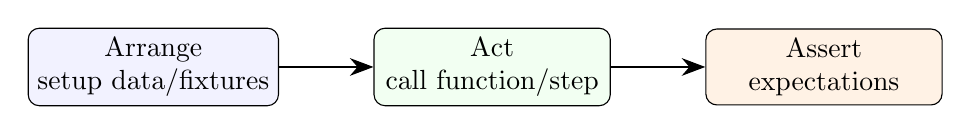
\begin{tikzpicture}[
  node distance=12mm,
  box/.style={draw, rounded corners, align=center, minimum width=30mm, minimum height=8mm},
  >={Stealth[length=3mm]}
]
  \node[box, fill=blue!5] (arrange) {Arrange\\setup data/fixtures};
  \node[box, fill=green!5, right=of arrange] (act) {Act\\call function/step};
  \node[box, fill=orange!10, right=of act] (assert) {Assert\\expectations};
  \draw[->] (arrange) -- (act);
  \draw[->] (act) -- (assert);
\end{tikzpicture}
\end{center}

\section*{Logging Basics}
Minimal logging setup:
\begin{lstlisting}[style=py]
import logging

logging.basicConfig(
    level=logging.INFO,
    format="%(asctime)s [%(levelname)s] %(name)s: %(message)s"
)
logger = logging.getLogger("demo")
logger.info("Hello logs")
\end{lstlisting}

Capture logs in tests with \texttt{caplog}:
\begin{lstlisting}[style=py]
def greet(name):
    logger = logging.getLogger("demo")
    logger.info("Greeting %s", name)
    return f"Hello, {name}!"

def test_greet_logs(caplog):
    caplog.set_level(logging.INFO, logger="demo")
    assert greet("Ada") == "Hello, Ada!"
    assert any("Greeting Ada" in rec.getMessage() for rec in caplog.records)
\end{lstlisting}

\section*{Selenium Waits (Reliable)}
Avoid \texttt{time.sleep}. Use explicit waits:
\begin{lstlisting}[style=py]
from selenium import webdriver
from selenium.webdriver.common.by import By
from selenium.webdriver.support.ui import WebDriverWait
from selenium.webdriver.support import expected_conditions as EC

driver = webdriver.Chrome()
driver.get("https://www.saucedemo.com/")

WebDriverWait(driver, 10).until(
    EC.visibility_of_element_located((By.ID, "user-name"))
).send_keys("standard_user")

WebDriverWait(driver, 10).until(
    EC.visibility_of_element_located((By.ID, "password"))
).send_keys("secret_sauce")

WebDriverWait(driver, 10).until(
    EC.element_to_be_clickable((By.ID, "login-button"))
).click()
\end{lstlisting}

\section*{Logging Flow Diagram}
\begin{center}
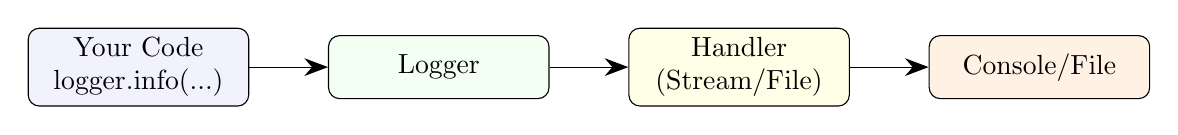
\begin{tikzpicture}[
  node distance=10mm,
  box/.style={draw, rounded corners, align=center, minimum width=28mm, minimum height=8mm},
  >={Stealth[length=3mm]}
]
  \node[box, fill=blue!5] (code) {Your Code\\logger.info(...) };
  \node[box, fill=green!5, right=of code] (logger) {Logger};
  \node[box, fill=yellow!10, right=of logger] (handler) {Handler\\(Stream/File)};
  \node[box, fill=orange!10, right=of handler] (output) {Console/File};
  \draw[->] (code) -- (logger);
  \draw[->] (logger) -- (handler);
  \draw[->] (handler) -- (output);
\end{tikzpicture}
\end{center}

\section*{Common Fixtures Cheat Sheet}
\begin{itemize}
  \item \textbf{caplog}: capture logging records.
  \item \textbf{tmp\_path}: temp directory per test.
  \item \textbf{monkeypatch}: override env/attributes for isolation.
  \item \textbf{capsys}: capture stdout/stderr.
\end{itemize}

\end{document}
